% !TEX program = lualatex
\documentclass[5p,10pt]{elsarticle}

\usepackage{luatexja}
\usepackage{luatexja-fontspec}
\usepackage{amsmath,amssymb}
\usepackage{graphicx}
\usepackage{booktabs}
\usepackage{multirow}
\usepackage{siunitx}
\usepackage{xcolor}
\usepackage[colorlinks=true,linkcolor=blue,citecolor=blue,urlcolor=blue]{hyperref}
\usepackage{longtable}
\usepackage{array}
\usepackage{float}
\usepackage{enumitem}
\usepackage{caption}
\captionsetup{font=small,labelfont=bf}
\usepackage{tikz}
\usetikzlibrary{arrows.meta,positioning,shapes.geometric}

\setlist{nosep,leftmargin=*}

% Japanese fonts
\setmainjfont{IPAexMincho}
\setsansjfont{IPAexGothic}

% Section numbering: S1, S2, ...
\renewcommand{\thesection}{S\arabic{section}}
\renewcommand{\thesubsection}{S\arabic{section}.\arabic{subsection}}
\renewcommand{\thetable}{S\arabic{table}}
\renewcommand{\thefigure}{S\arabic{figure}}
\renewcommand{\theequation}{S\arabic{equation}}

\journal{---}

\begin{document}

\begin{frontmatter}
\title{Supplementary Material:\\
DFT体積サイズファクターの元素別加法分解による\\
高エントロピー合金の格子定数予測}
\end{frontmatter}


\section{剛体球接触モデルの解析}
\label{sec:appendix_packing}

DFT格子定数から最近接距離を求め、剛体球接触モデルで
有効半径を評価する。
L1$_2$ $A_3B$では
\begin{equation}
  a^{\text{L1}_2} = \sqrt{2}\,\max(r_A + r_B,\; 2r_A),
  \label{eq:dnn_l12}
\end{equation}
B2では
\begin{equation}
  a^{\text{B2}} = \max\!\left(\frac{2(r_A + r_B)}{\sqrt{3}},\;
    2r_A,\; 2r_B\right)\!.
  \label{eq:dnn_b2}
\end{equation}
単一半径セットの全構造同時フィットは
RMSE = 0.162~\AA{}と大きく、剛体球仮定の破綻を示す。


\section{純元素原子体積のデータソース選択}
\label{sec:appendix_volumes}

King体積をDFT計算値に置き換える3つの試みを検証したが、
いずれもHEA格子定数の予測精度（RMSE）はKing値使用時を上回れなかった。

\subsection{VASP B2同種ペア体積}
\label{sec:appendix_vasp_homo}

VASP B2同種ペアから仮想BCC体積$V^A_\text{BCC} = a^3_\text{B2}/2$を取得。
31元素中$|\Delta| > 3$\%は11元素に及ぶ
（Mn: $-11$\%, Ag: $+5.4$\%等）。
GGA系統誤差が原因（Si・Ge・Bは安定構造がBCC/FCCでなく乖離が15--29\%に達するため全体から除外済）。
Vegard RMSE: 0.0231$\to$0.0348~\AA{}（51\%悪化）。

\begin{table}[H]
\centering
\caption{31元素のKing実験体積とVASP B2同種体積の比較（代表元素）。}
\label{tab:king_vs_vasp_bcc}
\footnotesize
\begin{tabular}{@{}lcrrr@{}}
\toprule
元素 & 安定構造 & King (\AA$^3$) & VASP BCC (\AA$^3$) & $\Delta$ (\%) \\
\midrule
Si$^*$  & diamond    & 20.02 & 14.81 & $\mathbf{-26.0}$ \\
Mn      & $\alpha$-Mn & 12.21 & 10.84 & $\mathbf{-11.2}$ \\
Ag      & FCC        & 17.06 & 17.98 & $\mathbf{+5.4}$ \\
Cr      & BCC        & 12.01 & 11.41 & $\mathbf{-5.0}$ \\
Fe      & BCC        & 11.78 & 11.29 & $\mathbf{-4.1}$ \\
Al      & FCC        & 16.60 & 16.78 & $+1.1$ \\
Ni      & FCC        & 10.94 & 10.90 & $-0.3$ \\
Mo      & BCC        & 15.58 & 15.61 & $+0.2$ \\
\bottomrule
\end{tabular}
\par\smallskip
{\scriptsize $^*$Si・Ge・Bは安定構造がBCC/FCCでなく乖離が極端なため全体から除外済。参考として掲載。}
\end{table}

\subsection{Wang (2004) ab initio安定構造体積}
\label{sec:appendix_wang}

Wang~\cite{Wang2004lattice}の安定構造体積を用いても
Vegard RMSE = 0.0338~\AA{}（King: 0.0227~\AA{}）、
最適$q$でもRMSE = 0.0320~\AA{}。
$q_\text{FCC} = -0.47$と非物理的値を示す。

\begin{table}[H]
\centering
\caption{$V_i$ソース別のHEA予測精度（64 HEA）。
  King実験値が全DFT代替案を上回る。}
\label{tab:vi_comparison}
\footnotesize
\begin{tabular}{@{}lcccc@{}}
\toprule
$V_i$ソース & Vegard RMSE & 最適$q$ RMSE & $q_\text{BCC}$ & $q_\text{FCC}$ \\
\midrule
\textbf{King実験値}  & \textbf{0.0227} & \textbf{0.0214} & 0.49 & 0.13 \\
Wang安定構造~\cite{Wang2004lattice}   & 0.0338 & 0.0320 & 0.75 & $-0.47$ \\
Wang BCC     & 0.0359 & 0.0342 & 0.85 & 0.03 \\
VASP B2同種  & 0.0348 & 0.0258 & 0.56 & $-0.62$ \\
\bottomrule
\end{tabular}
\end{table}

\subsection{DFT体積が劣る根本原因}
\label{sec:appendix_dft_limitation}

GGA-PBEの元素依存系統誤差（Au: $+7.1$\%, Fe: $-4.6$\%等）が
Vegardベースラインを直接劣化させる。
$\Omega_\text{sf}$は比として定義されるため
GGA誤差が部分的に相殺されるのに対し、
$V_i$は格子体積を直接決定するため影響が大きい。
これがKing $V_i$ + DFT $\Omega_\text{sf}$ + $q$の
混合アプローチの優位性の物理的根拠である。


\section{VASP B2/L1$_2$データ統合の分析}
\label{sec:appendix_vasp}

VASP B2（2,200計算、2,136収束）・
L1$_2$（2,810計算、2,169収束）の統合により
カバレッジはB2: 152$\to$465ペア、L1$_2$: 95$\to$441ペアに拡大（4f希土類+Y除外後）。
HEA予測に必要な全ペアのDFT $\Omega_\text{sf}$が
利用可能となった（BCC 10/59$\to$59/59、FCC 4/42$\to$42/42）。


\section{その他の留意事項}
\label{sec:appendix_notes}

\subsection{$4f$希土類+Y除外の理由}
\label{sec:appendix_gdce}

$4f$希土類14元素（La, Ce, Pr, Nd, Sm, Eu, Gd, Tb, Dy, Ho, Er, Tm, Yb, Lu）およびYは、
GGA-PBEが$4f$局在電子を正しく扱えず、格子定数が非物理的に膨張（$a \approx 4.000$~\AA{}で停止）または
発散（$a > 5.5$~\AA）するため全解析から除外した。
$\Omega_\text{sf}$に最大$+3.4$の異常値が混入し、L1$_2$非対称性相関を$r = 0.02$に希釈していた。
除外後は$r = 0.71$に回復し、B2 $R^2$は0.43$\to$0.56、L1$_2$ $R^2$は0.20$\to$0.66と大幅に改善した。
HEA予測に使用する21元素には4f元素を含まないため、予測精度への影響はない。
DFT+$U$やハイブリッド汎関数の適用が今後の課題である。

\subsection{温度効果}

DFTは0~K格子定数を与えるが実験値は室温測定。
King体積は室温値のためVegard基準線と温度整合する。
$\Omega_\text{sf}$は偏差の比として定義されるため
温度効果が部分的に相殺されるが、
BCC HEAでは線膨張係数の元素間差が大きく
温度補正が精度改善に寄与する可能性がある。

\subsection{加法分解の精度上限}

加法$\delta_i + \delta_j$分解で全分散の34--44\%が失われるが（B2: $R^2 = 0.56$、L1$_2$: $R^2 = 0.66$）、
HEA予測ではRMSE = 0.0221~\AA{}（元素対: 0.0214~\AA）と
実用上の問題はない。
残差は元素対固有の電荷移動・磁気相互作用に起因し、
加法性仮定の本質的限界を反映する。


%% =====================================================================
\section{記号一覧}
\label{sec:nomenclature}
%% =====================================================================

\begin{table}[H]
\centering
\caption{本論文で用いる主要記号。}
\label{tab:nomenclature}
\footnotesize
\begin{tabular}{@{}lll@{}}
\toprule
記号 & 定義 & 単位 \\
\midrule
$a$ & 格子定数 & \AA \\
$V_i$ & 元素$i$のKing原子体積 & \AA$^3$ \\
$c_i$ & 元素$i$の原子分率 & --- \\
$n_\text{auc}$ & 単位胞あたり原子数（BCC: 2, FCC: 4） & --- \\
$\Omega_\text{sf}^{(s)}(i\text{-}j)$ & 構造$s$での体積サイズファクター & --- \\
$\delta_i^{(s)}$ & 元素$i$の加法分解パラメータ（構造$s$） & --- \\
$q_s$ & 構造依存校正定数 & --- \\
$V_\text{eff}(i;\,\mathbf{c})$ & 組成依存有効原子体積 & \AA$^3$ \\
$\delta r$ & 原子サイズミスマッチパラメータ & \% \\
$\alpha$ & Warren-Cowley短距離秩序パラメータ & --- \\
\midrule
\multicolumn{3}{@{}l}{\textit{略語}} \\
HEA & 高エントロピー合金 (High-Entropy Alloy) & \\
DFT & 密度汎関数理論 (Density Functional Theory) & \\
VASP & Vienna Ab initio Simulation Package & \\
GGA-PBE & 一般化勾配近似（Perdew-Burke-Ernzerhof） & \\
SQS & Special Quasi-random Structure & \\
LOO-CV & Leave-One-Out交差検証 & \\
RMSE & 二乗平均平方根誤差 & \AA \\
MAE & 平均絶対誤差 & \AA \\
GPR & ガウス過程回帰 (Gaussian Process Regression) & \\
XGBoost & eXtreme Gradient Boosting & \\
\bottomrule
\end{tabular}
\end{table}


%% =====================================================================
\section{格子定数予測の計算例}
\label{sec:appendix_examples}
%% =====================================================================

本付録では、本文の手法を用いて実際のHEAの格子定数を
手計算で予測する手順を示す。
読者はスプレッドシート等で追試可能である。

\subsection{例題1: CoCrFeNi（FCC HEA）--- L1$_2$参照}
\label{sec:example_fcc}

等モル4元系FCC HEA CoCrFeNiの格子定数を予測する。

\paragraph{Step 1: King原子体積の取得}

表~\ref{tab:delta_params}または文献~\cite{King1966}より：
\begin{align*}
V_\text{Co} &= 11.073~\text{\AA}^3, & V_\text{Cr} &= 12.008~\text{\AA}^3, \\
V_\text{Fe} &= 11.776~\text{\AA}^3, & V_\text{Ni} &= 10.941~\text{\AA}^3.
\end{align*}

\paragraph{Step 2: Vegard則による計算}

等モル（$c_i = 0.25$）、FCC（$n_\text{auc} = 4$）：
\begin{align}
V_\text{Vegard} &= \sum_i c_i V_i = 0.25(11.073 + 12.008 + 11.776 + 10.941) \nonumber \\
&= 11.450~\text{\AA}^3, \nonumber \\
a_\text{Vegard} &= (4 \times 11.450)^{1/3} = 3.578~\text{\AA}. \label{eq:ex_vegard_fcc}
\end{align}

\paragraph{Step 3: L1$_2$~$\Omega_\text{sf}$の取得}

$\binom{4}{2} = 6$ペアのDFT $\Omega_\text{sf}^{\text{L1}_2}$：
\begin{center}
\footnotesize
\begin{tabular}{@{}lrlr@{}}
\toprule
ペア & $\Omega_\text{sf}$ & ペア & $\Omega_\text{sf}$ \\
\midrule
Co--Cr & $-0.047$ & Cr--Ni & $-0.032$ \\
Co--Fe & $-0.017$ & Fe--Ni & $-0.004$ \\
Co--Ni & $-0.014$ & Cr--Fe & $-0.057$ \\
\bottomrule
\end{tabular}
\end{center}

\paragraph{Step 4: 本文式(7)による補正}

$q_\text{FCC} = 0.13$で二重和を計算する：
\begin{equation}
\text{補正項} = \sum_i \sum_{j \ne i} c_i\,c_j\,V_j\,\Omega_\text{sf}^{\text{L1}_2}(i,j)
= -0.247~\text{\AA}^3.
\label{eq:ex_correction_fcc}
\end{equation}
全体の体積と格子定数：
\begin{align}
V &= 4 \times (11.450 + 0.13 \times (-0.247)) = 45.67~\text{\AA}^3, \nonumber \\
a_\text{pred} &= V^{1/3} = 3.573~\text{\AA}. \label{eq:ex_pred_fcc}
\end{align}

\paragraph{Step 5: 実験値との比較}

$a_\text{exp} = 3.575$~\AA{}（Alonso Table~2）。
誤差 $= |3.574 - 3.575| = 0.001$~\AA{}。
Vegard（$a = 3.578$~\AA、誤差0.003~\AA）よりも実験値に近い。

\medskip
\noindent
全$\Omega_\text{sf}$が負（収縮方向）であることは、
3$d$遷移金属間の強い$d$--$d$結合が
単純体積加算（Vegard）よりも密なパッキングを生むことを反映している。


\subsection{例題2: HfNbTaTiZr（BCC HEA）--- B2参照}
\label{sec:example_bcc}

等モル5元系BCC HEA HfNbTaTiZr（Senkov合金）の格子定数を予測する。

\paragraph{Step 1: King原子体積}
\begin{align*}
V_\text{Hf} &= 22.312~\text{\AA}^3, & V_\text{Nb} &= 17.978~\text{\AA}^3, \\
V_\text{Ta} &= 18.014~\text{\AA}^3, & V_\text{Ti} &= 17.649~\text{\AA}^3, \\
V_\text{Zr} &= 23.279~\text{\AA}^3. &
\end{align*}

\paragraph{Step 2: Vegard則}

等モル（$c_i = 0.20$）、BCC（$n_\text{auc} = 2$）：
\begin{align}
V_\text{Vegard} &= 0.20 \times (22.312 + 17.978 + 18.014 + 17.649 + 23.279) \nonumber \\
&= 19.846~\text{\AA}^3, \nonumber \\
a_\text{Vegard} &= (2 \times 19.846)^{1/3} = 3.411~\text{\AA}. \label{eq:ex_vegard_bcc}
\end{align}

\paragraph{Step 3: B2~$\Omega_\text{sf}$}

$\binom{5}{2} = 10$ペアのDFT $\Omega_\text{sf}^\text{B2}$：
\begin{center}
\footnotesize
\begin{tabular}{@{}lrlr@{}}
\toprule
ペア & $\Omega_\text{sf}$ & ペア & $\Omega_\text{sf}$ \\
\midrule
Hf--Nb & $-0.013$ & Nb--Ti & $-0.028$ \\
Hf--Ta & $-0.015$ & Nb--Zr & $-0.018$ \\
Hf--Ti & $-0.023$ & Ta--Ti & $-0.028$ \\
Hf--Zr & $-0.016$ & Ta--Zr & $-0.020$ \\
Nb--Ta & $+0.017$ & Ti--Zr & $-0.030$ \\
\bottomrule
\end{tabular}
\end{center}

\paragraph{Step 4: B2参照での予測（$q_\text{BCC} = 0.49$）}
\begin{align}
\text{補正項} &= \sum_i \sum_{j \ne i} c_i\,c_j\,V_j\,\Omega_\text{sf}^\text{B2}(i,j)
= -0.280~\text{\AA}^3, \nonumber \\
V &= 2 \times (19.846 + 0.49 \times (-0.280)) = 39.42~\text{\AA}^3, \nonumber \\
a_\text{pred}^{\text{B2}} &= 39.43^{1/3} = 3.403~\text{\AA}. \label{eq:ex_pred_bcc}
\end{align}

\paragraph{Step 5: 実験値との比較}

$a_\text{exp} = 3.410$~\AA{}（Senkov 2012）。
誤差 $= |3.403 - 3.410| = 0.007$~\AA。
Vegard（$a = 3.411$~\AA、誤差0.001~\AA）と比較すると本例ではVegardが偶然よい。
この合金は$\Omega_\text{sf}$のほとんどが負（収縮方向）であり
$q < 1$の補正がVegard側に引き戻す効果が不十分な例である。

\paragraph{補足: SQS参照（$q = 1$）の場合}
SQS $\Omega_\text{sf}$を用いると補正量が小さくなり
$a_\text{pred}^{\text{SQS}} \approx 3.41$~\AA{}となる。
B2の秩序効果（$\alpha = -1$）による$\Omega_\text{sf}$の過大評価が
SQS（$\alpha \approx 0$）で解消されるためである。


%% =====================================================================
\section{$\delta^{(s)}$パラメータ一覧}
\label{sec:appendix_delta}
%% =====================================================================

表~\ref{tab:delta_params}に31元素の加法分解パラメータ$\delta_i^{(s)}$を示す。
任意の$N$元HEA（BCC/FCC）について、
本表の$\delta$値とKing原子体積$V_i$のみで本文式(9)により
格子定数を予測できる。

\begin{table*}[!t]
\centering
\caption{31元素の加法分解パラメータ$\delta^{(s)}$およびKing原子体積。
$\delta^\text{B2}$はBCC HEA予測に、$\delta^{\text{L1}_2}$はFCC HEA予測に使用する。}
\label{tab:delta_params}
\footnotesize
\begin{tabular}{@{}lrrr|lrrr@{}}
\toprule
元素 & $V_i$ (\AA$^3$) & $\delta^\text{B2}$ & $\delta^{\text{L1}_2}$ &
元素 & $V_i$ (\AA$^3$) & $\delta^\text{B2}$ & $\delta^{\text{L1}_2}$ \\
\midrule
Ag &  17.061 & $+$0.041 & $+$0.030 & Os &  13.977 & $-$0.011 & $-$0.005 \\
Al &  16.602 & $-$0.041 & $-$0.027 & Pb &  30.321 & $-$0.045 & $-$0.033 \\
Au &  16.966 & $+$0.038 & $+$0.034 & Pd &  14.716 & $+$0.024 & $+$0.012 \\
Be &   8.111 & $+$0.003 & $+$0.000 & Pt &  15.095 & $+$0.018 & $+$0.008 \\
Ca &  43.630 & $-$0.180 & $-$0.175 & Re &  14.712 & $-$0.016 & $-$0.020 \\
Co &  11.073 & $-$0.032 & $-$0.031 & Rh &  13.754 & $+$0.003 & $-$0.009 \\
Cr &  12.008 & $+$0.031 & $-$0.001 & Ru &  13.571 & $-$0.012 & $-$0.008 \\
Cu &  11.810 & $+$0.007 & $+$0.009 & Sc &  24.987 & $-$0.071 & $-$0.049 \\
Fe &  11.776 & $-$0.035 & $-$0.029 & Sn &  27.053 & $-$0.076 & $-$0.050 \\
Hf &  22.312 & $-$0.027 & $-$0.016 & Ta &  18.014 & $-$0.006 & $+$0.003 \\
Ir &  14.155 & $+$0.003 & $-$0.006 & Ti &  17.649 & $-$0.037 & $-$0.027 \\
Mg &  23.240 & $-$0.084 & $-$0.066 & V  &  13.824 & $-$0.003 & $-$0.009 \\
Mn &  12.210 & $-$0.004 & $-$0.013 & W  &  15.850 & $-$0.012 & $-$0.001 \\
Mo &  15.583 & $-$0.007 & $+$0.000 & Zn &  15.207 & $-$0.019 & $-$0.019 \\
Nb &  17.978 & $+$0.006 & $+$0.016 & Zr &  23.279 & $-$0.019 & $-$0.018 \\
Ni &  10.941 & $-$0.014 & $-$0.016 &    &         &          &          \\
\bottomrule
\end{tabular}
\end{table*}

\noindent
使用法：任意のHEA（元素$\{i\}$、組成$\{c_i\}$、構造$s$）の格子定数を以下で予測する。
\begin{enumerate}
  \item 構造$s$を選択（BCC: $\delta^\text{B2}$使用、FCC: $\delta^{\text{L1}_2}$使用）。
  \item 各元素の有効体積を計算：
    $V_\text{eff}(i) = V_i\,[1 + q_s \sum_{j \ne i} c_j\,(\delta_i^{(s)} + \delta_j^{(s)})]$。
  \item 格子定数を求める：
    $a = (n_\text{auc} \sum_i c_i\,V_\text{eff}(i))^{1/3}$。
\end{enumerate}
校正定数: $q_\text{BCC} = 0.49$（B2参照）または$1.0$（SQS参照）、$q_\text{FCC} = 0.13$。


%% =====================================================================
%% Supplementary: Vegard則の全ペア検証
%% =====================================================================

\section{全元素ペアにおけるVegard則の成立度}
\label{sec:appendix_vegard_all}

本文§3.3では代表6ペアで構造整合Vegard検証を行った。
ここでは全元素ペアに対する系統的検証の結果を示す。
すべての図においてDFT同種体積
（B2: $V_X^\text{BCC} = a_\text{B2}(X\text{-}X)^3/2$、
L1$_2$: $V_X^\text{FCC} = a_{\mathrm{L1}_2}(X\text{-}X)^3/4$）
を構造整合端点として使用している。

\subsection{$\Omega_\text{sf}$ヒートマップ}

図~\ref{fig:vegard_heatmap_b2}・\ref{fig:vegard_heatmap_l12}に
全ペアの$\Omega_\text{sf}$を元素$\times$元素の行列として示す。
B2（図~\ref{fig:vegard_heatmap_b2}）では
大半のペアが負の$\Omega_\text{sf}$（体積収縮）を示し、
B2秩序構造における系統的なVegard過大評価が確認される。
L1$_2$（図~\ref{fig:vegard_heatmap_l12}）では
Dy, Er, Tb, Sm等の希土類4f元素が行・列全体にわたって
極端な正の偏差を示す。
これはGGA-PBEが4f局在電子の体積を過大評価するためであり、
これらの元素を含むペアの$\Omega_\text{sf}$は
物理的に信頼できない。

\begin{figure*}[!t]
\centering
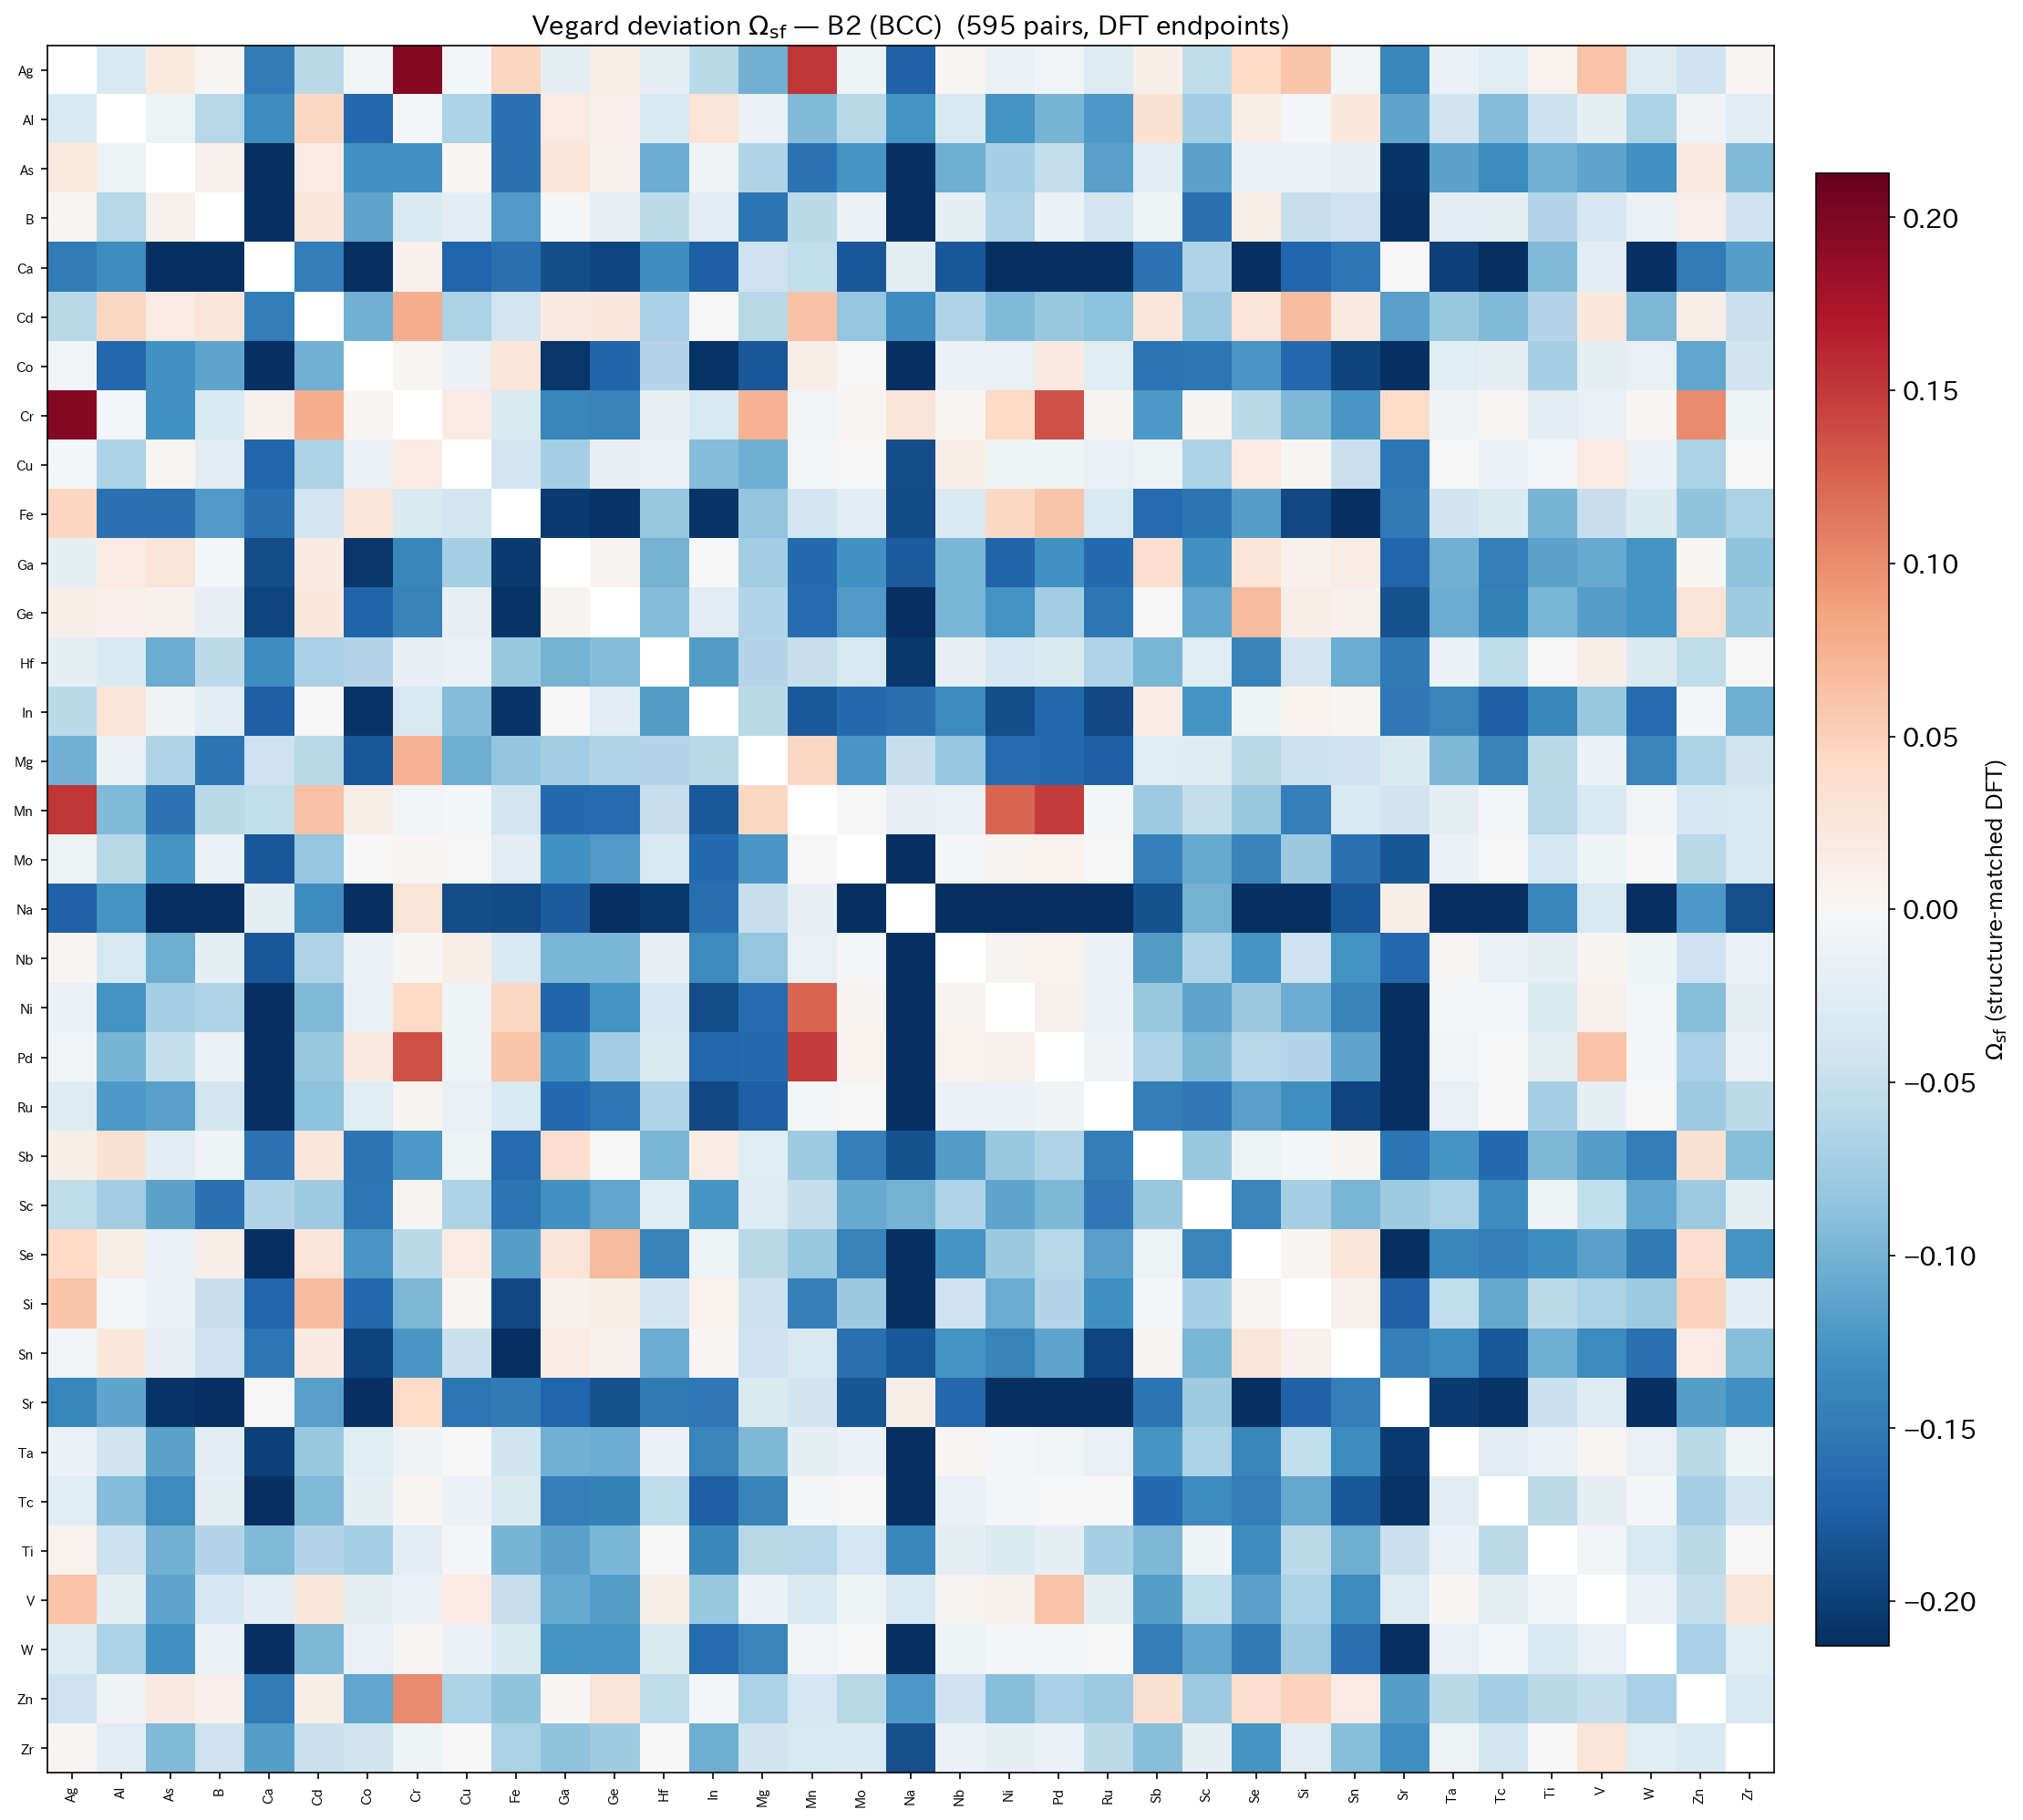
\includegraphics[width=\textwidth]{fig_vegard_heatmap_b2.png}
\caption{全元素ペアのB2（BCC型）$\Omega_\text{sf}$ヒートマップ
  （465ペア、31元素）。
  DFT B2同種体積を端点としたVegard偏差。
  青: 体積収縮（$\Omega_\text{sf} < 0$）、
  赤: 体積膨張（$\Omega_\text{sf} > 0$）。
  大半のペアが負の偏差を示し、B2秩序構造における体積収縮傾向を反映する。}
\label{fig:vegard_heatmap_b2}
\end{figure*}

\begin{figure*}[!t]
\centering
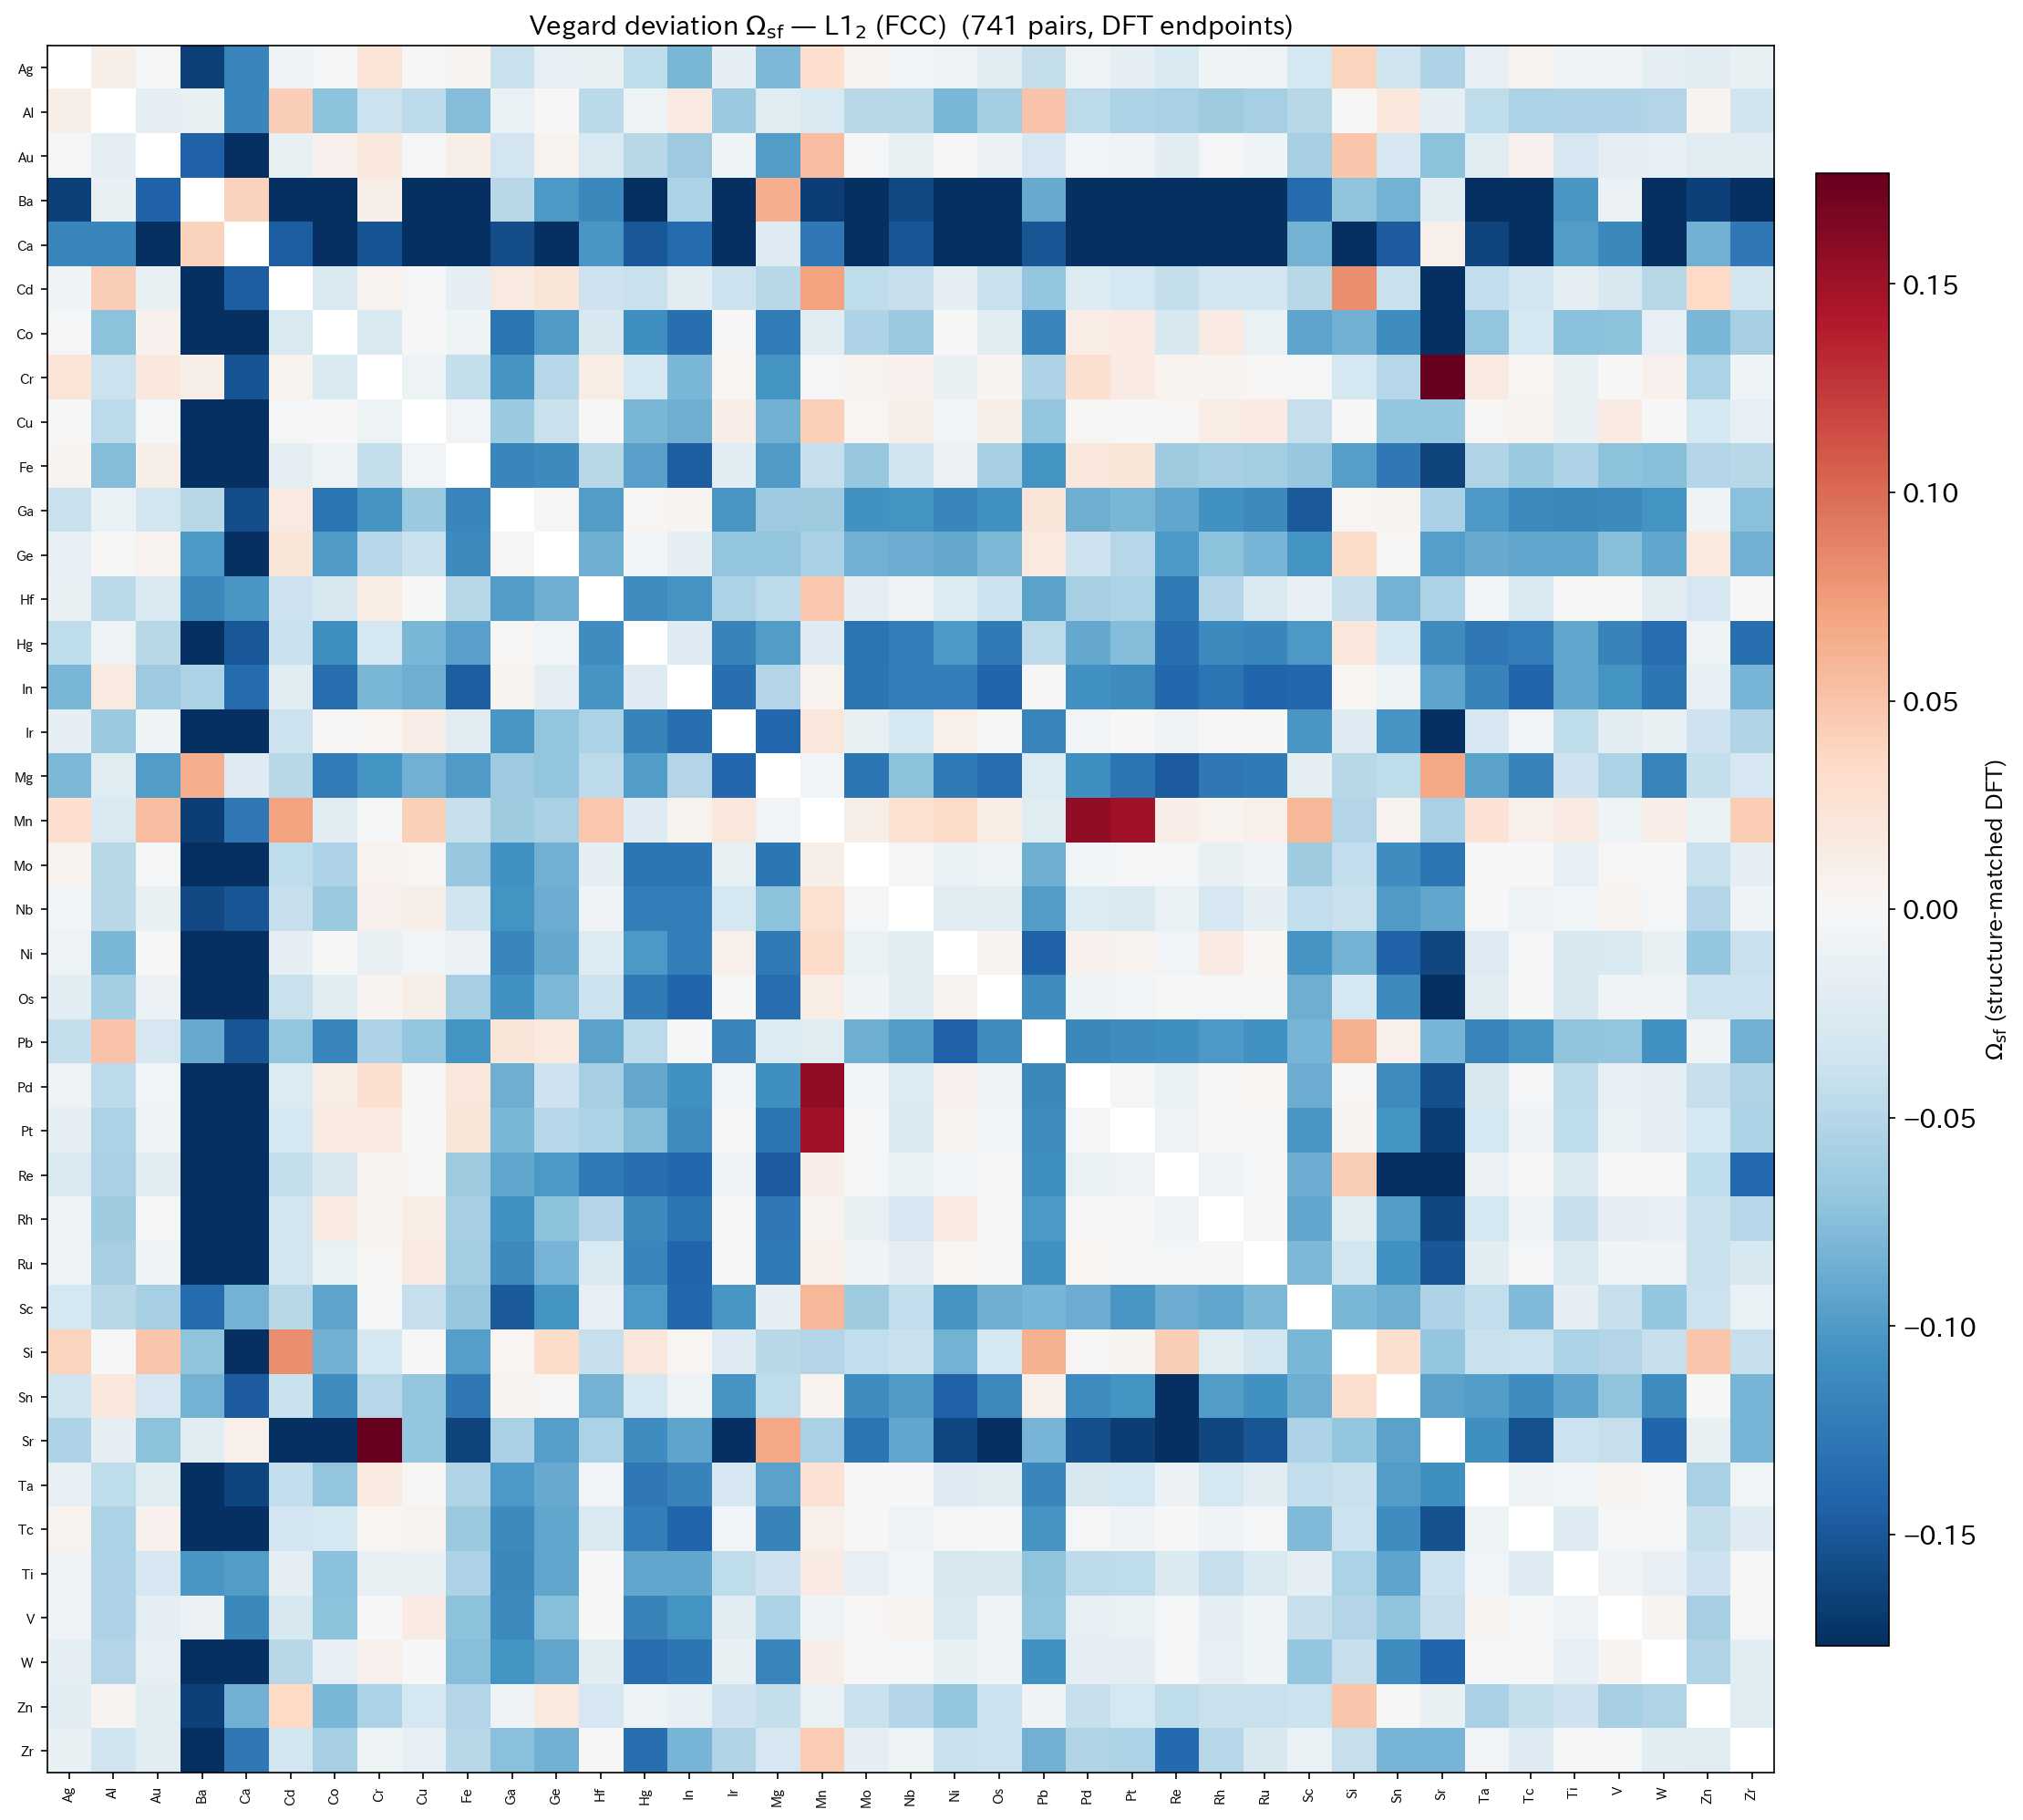
\includegraphics[width=\textwidth]{fig_vegard_heatmap_l12.png}
\caption{全元素ペアのL1$_2$（FCC型）$\Omega_\text{sf}$ヒートマップ
  （1275ペア、51元素）。
  DFT L1$_2$同種体積を端点としたVegard偏差。
  Dy, Er, Tb, Sm等の希土類4f元素が行・列で極端な正の偏差を示す。}
\label{fig:vegard_heatmap_l12}
\end{figure*}

\subsection{Vegardパリティプロット（体積空間）}

図~\ref{fig:vegard_parity_b2}・\ref{fig:vegard_parity_l12}に
DFT原子体積$V_\text{DFT}$と構造整合Vegard予測体積
$V_\text{Vegard}$のパリティプロットを示す。
B2では$R^2 = 0.81$（RMSE = 2.50~\AA$^3$/atom、2045点）と
Vegard則が比較的良好に成立する。
一方、L1$_2$では$R^2 = 0.51$（RMSE = 5.34~\AA$^3$/atom、3148点）
と散乱が大きい。
L1$_2$の精度低下には2つの要因がある。
第一に、A$_3$B/B$_3$Aの非対称性により同一ペアでも
$\Omega_\text{sf}$が大きく異なる。
第二に、4f希土類元素のDFT体積異常が系統的な外れ値を生む。
B2が相対的に高精度である理由は、
c = 50\%の1点のみ（対称組成）であり
非線形効果が最大となる組成に限定されるためである。

\begin{figure*}[!t]
\centering
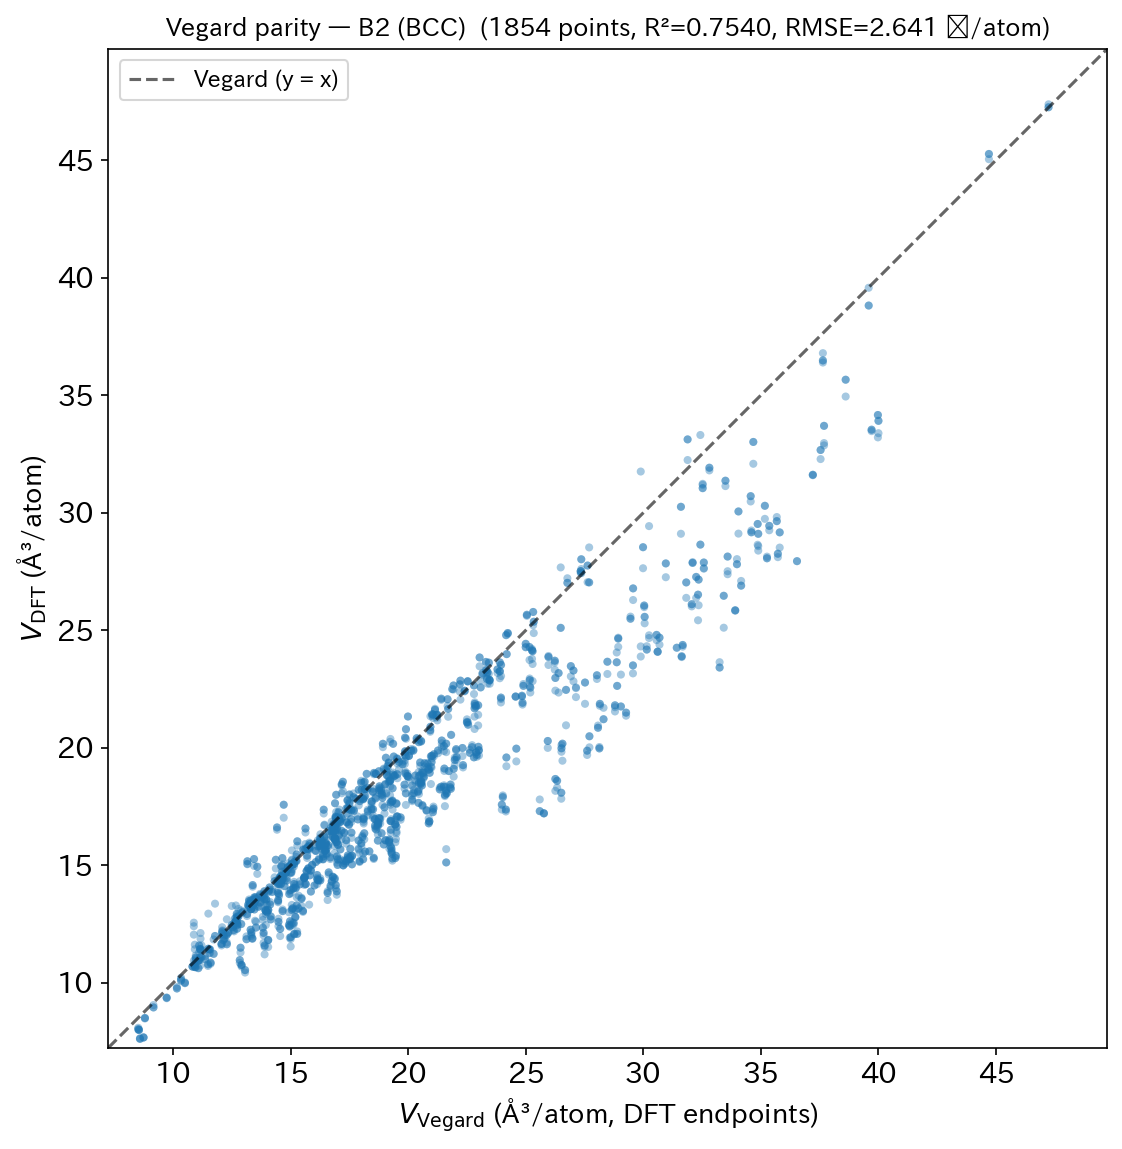
\includegraphics[width=0.7\textwidth]{fig_vegard_parity_b2.png}
\caption{全B2ペアのVegardパリティプロット
  （2045点、$R^2 = 0.81$、RMSE = 2.50~\AA$^3$/atom）。
  横軸: 構造整合DFT端点によるVegard予測体積、
  縦軸: DFT計算体積。破線はy = x（Vegard完全成立）。}
\label{fig:vegard_parity_b2}
\end{figure*}

\begin{figure*}[!t]
\centering
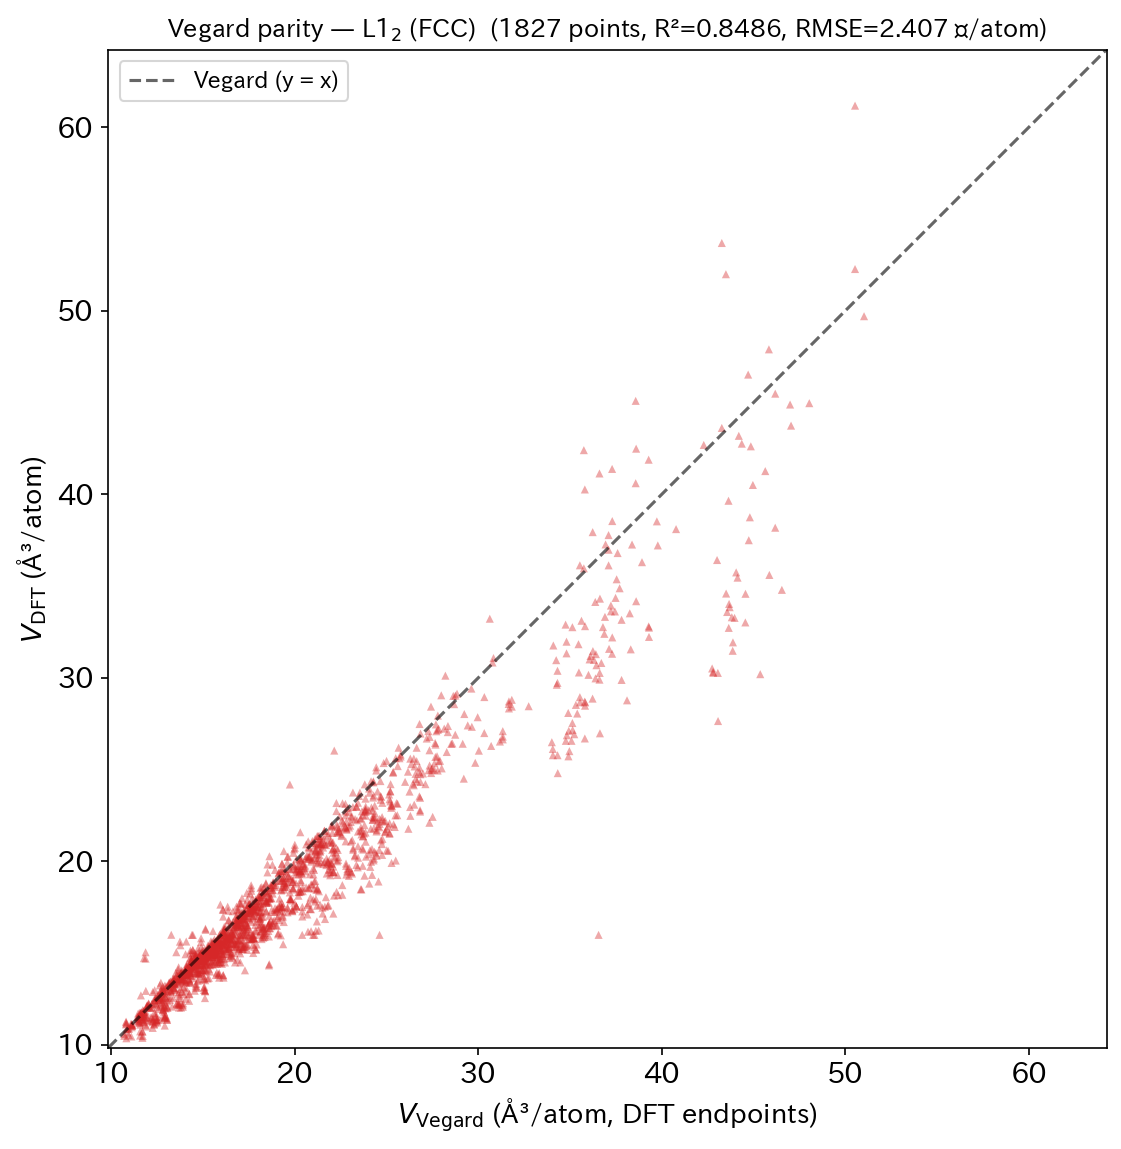
\includegraphics[width=0.7\textwidth]{fig_vegard_parity_l12.png}
\caption{全L1$_2$ペアのVegardパリティプロット
  （3148点、$R^2 = 0.51$、RMSE = 5.34~\AA$^3$/atom）。
  B2に比べ散乱が大きく、4f希土類の異常点が上方に突出する。}
\label{fig:vegard_parity_l12}
\end{figure*}

\subsection{$\Omega_\text{sf}$と原子半径差の関係}

図~\ref{fig:vegard_vs_radius_b2}・\ref{fig:vegard_vs_radius_l12}に
$\Omega_\text{sf}$を純元素のDFT半径差
$|\Delta r_\text{DFT}| = |r_A - r_B|$
（$r = (3V/4\pi)^{1/3}$で体積から変換）に対してプロットした。
B2では弱い負の相関（$r = -0.45$）があり、
サイズ差が大きいほど体積収縮（負の$\Omega_\text{sf}$）が
増大する傾向を示す。
これは異種原子間の電荷移動や$d$軌道結合が
サイズ差の大きいペアでより顕著であることと整合する。
L1$_2$では相関がさらに弱く（$r = -0.17$）、
$\Omega_\text{sf}$がサイズ差だけでは説明できない。
L1$_2$固有のA$_3$B/B$_3$A非対称性と
4f元素の異常が相関を希釈していると考えられる。

以上の結果は、$\Omega_\text{sf}$が単純なサイズ効果を超えた
電子構造由来の体積変化を含むことを示しており、
DFT計算による構造依存有効体積の導出が
Vegard則の補正に不可欠であることを裏付ける。

\begin{figure*}[!t]
\centering
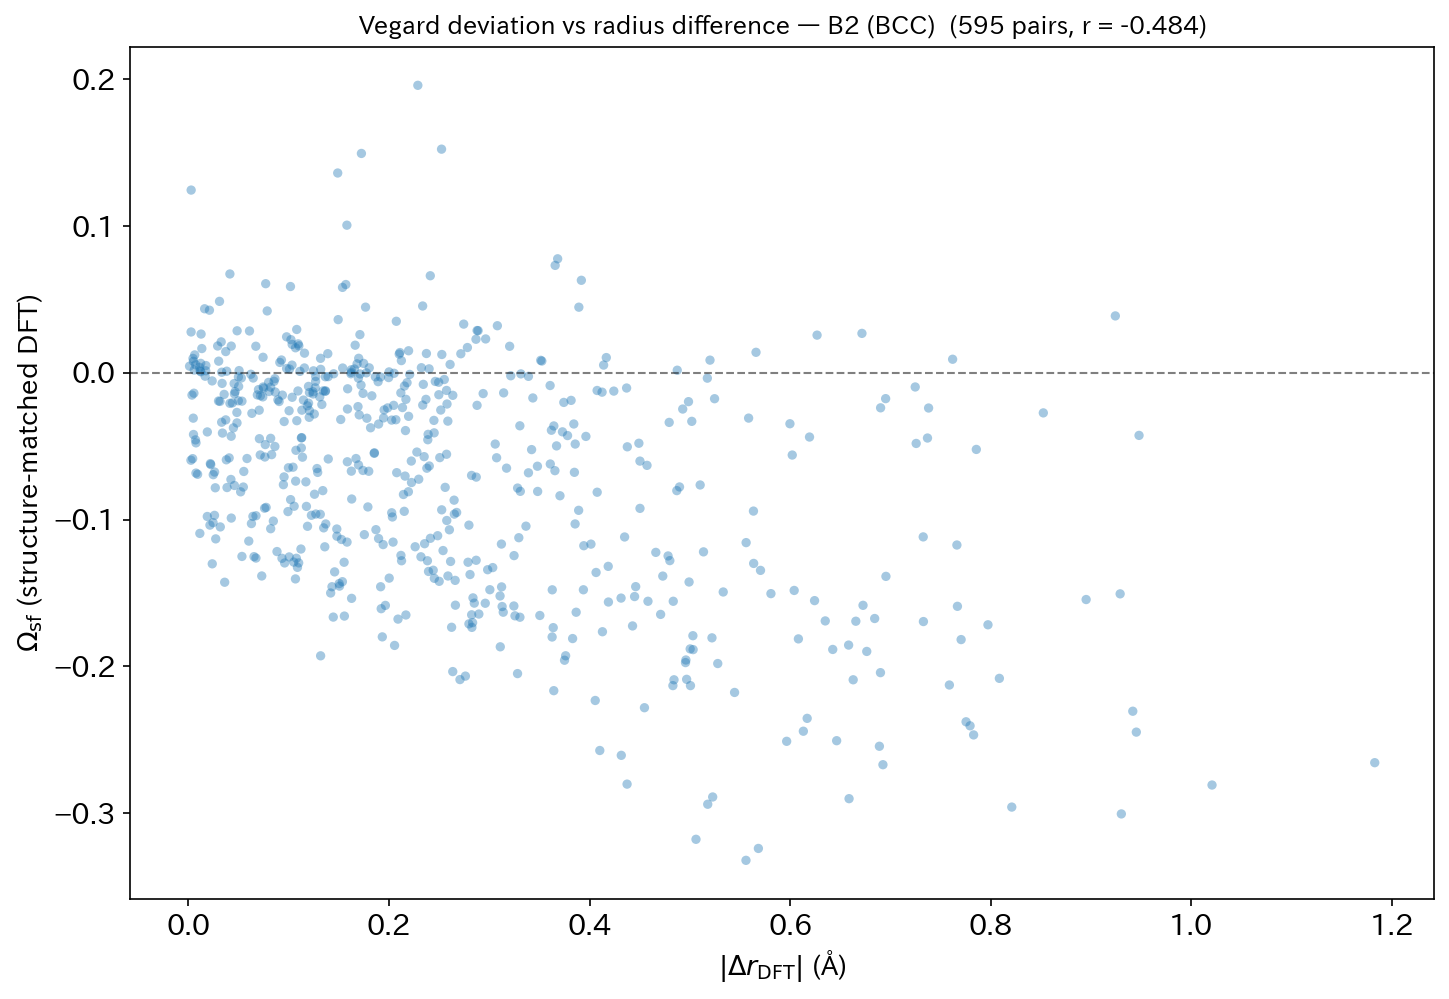
\includegraphics[width=0.7\textwidth]{fig_vegard_vs_radius_b2.png}
\caption{B2 $\Omega_\text{sf}$と純元素DFT半径差の関係
  （465ペア、$r = -0.45$）。
  半径差が大きいほど体積収縮（負の$\Omega_\text{sf}$）が増大する傾向。}
\label{fig:vegard_vs_radius_b2}
\end{figure*}

\begin{figure*}[!t]
\centering
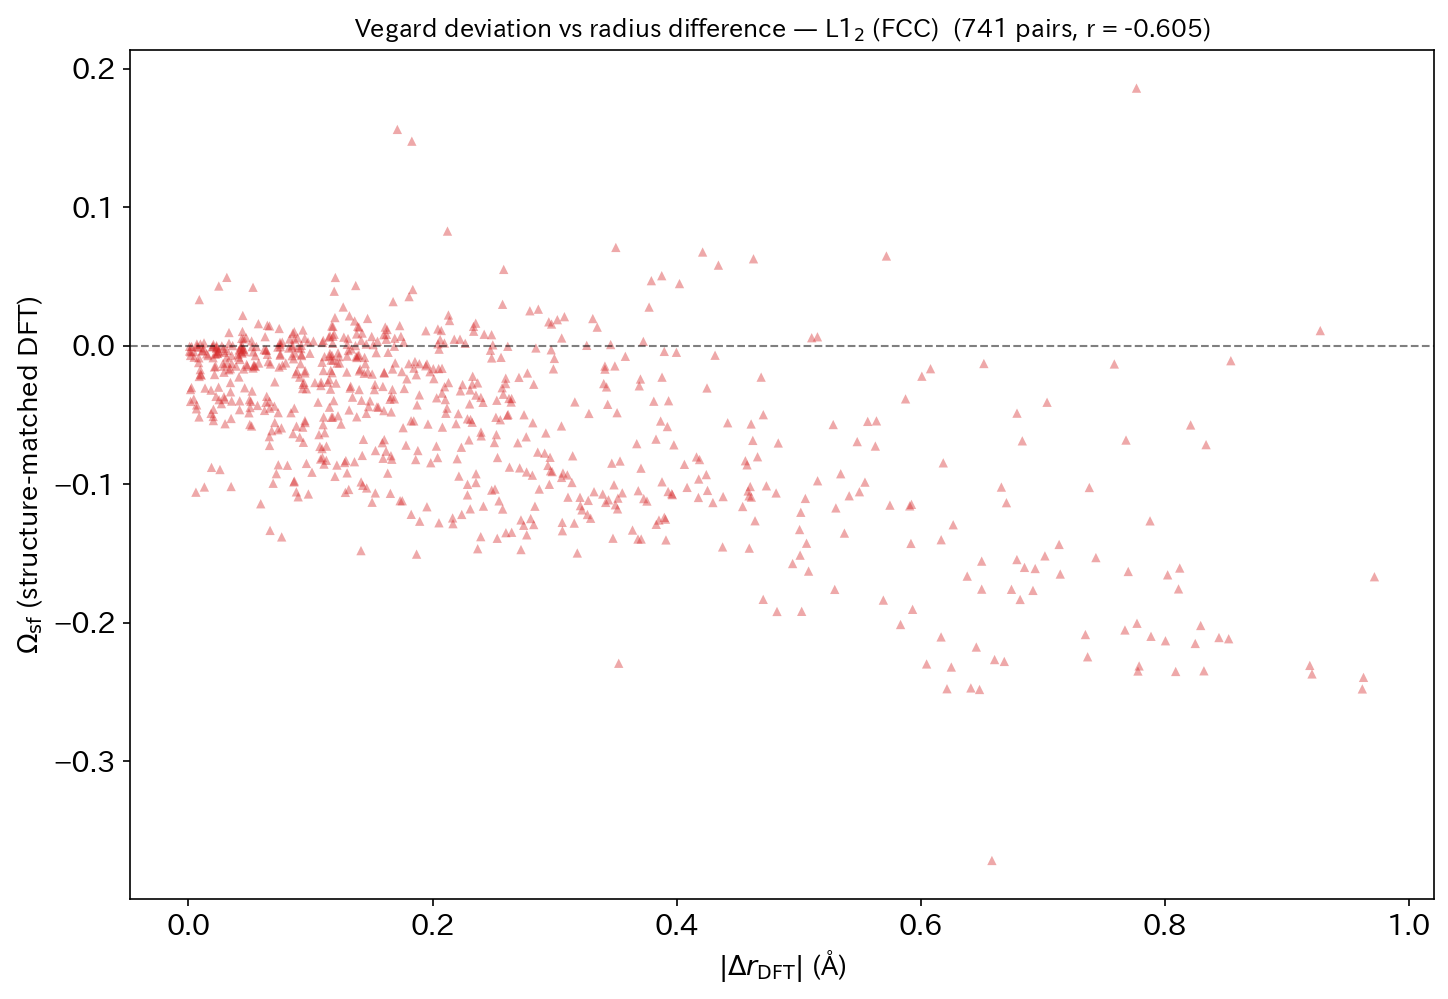
\includegraphics[width=0.7\textwidth]{fig_vegard_vs_radius_l12.png}
\caption{L1$_2$ $\Omega_\text{sf}$と純元素DFT半径差の関係
  （1275ペア、$r = -0.17$）。
  B2に比べ相関が弱く、$\Omega_\text{sf}$はサイズ差だけでは説明できない。}
\label{fig:vegard_vs_radius_l12}
\end{figure*}



\bibliographystyle{elsarticle-num}
\bibliography{references}

\end{document}
